As we revisit the Mumford-Shah Functional, we also rewrite Definition \ref{def:the_mumford_shah_functional} to be consistend with \cite{Pock-et-al-iccv09}, which is the publication we mainly follow in this chapter. If other results are taking into account, we make this clear.

\begin{definition}[Mumford-Shah Functional] % (fold)
\label{def:the_mumford_shah_functional_revisited}

    Let $\Omega \subset \mathbb{R}^{2}$ be a rectangular image domain. In order to approximate an input image $f: \Omega \longrightarrow \mathbb{R}$ in terms of a piecewise smooth function $u: \Omega \longrightarrow \mathbb{R}$, Mumford and Shah suggested to minimize the functional
        
        \begin{equation}
            E(u) = \lambda \int_{\Omega} (f - u)^{2} dx + \int_{\Omega \setminus S_{u}} |\nabla u|^{2} dx + \nu \mathcal{H}^{1}(S_{u}),
        \end{equation}
        \label{eq:the_mumford_shah_functional_revisited}
    
    where $\lambda, \nu > 0$ are weighting parameters, $S_{u} = S^{1}_{u} \cup ... \cup S^{N}_{u}$ and $\mathcal{H}^{1}(S_{u})$ denotes the n-1-dimensional Hausdorff-measure of the curves in $S_{u}$.

\end{definition}
% definition the_mumford_shah_functional (end)

The difference to Chapter 3 is, that we interchanged the set $K = K_{1} \cup ... \cup K_{N}$ to $S_{u} = S^{1}_{u} \cup ... \cup S^{N}_{u}$ and instead of computing $|K|$ the length of the curves we use the more general notation of measure theory. In the discrete case, the n-1-dimensional Hausdorff-measure of $S_{u}$ is nothing but $|S_{u}|$. And the parameter which handles the tradeoff between the data fidelity term and the gradient based term is swapped. So both definitions are totally consistent. As mentioned in the previous chapter, this functional is highly non-convex. The idea of \cite{Pock-et-al-iccv09} was to use convex relaxation techniques to derive a convex formulation of the Mumford-Shah functional. Then we would again be able to apply our fast primal-dual algorithm.

\section{Convex Relaxation} % (fold)
\label{sec:convex_relaxation}

    What we are looking for is the (global) minimal value of the piecewise smooth Mumford-Shah functional, i.e. $\min\limits_{u \in X} E(u)$. Another approach would be to minimize the piecewise constant functional where we set the weight $\lambda = \infty$, which we also discussed in the last chapter. In order to find a convex relaxation we need to introduce the characteristic function.

    \begin{definition}
    \label{def:characteristic_function}
        Let $\Omega \subset \mathbb{R}^{2}$ denote the image plane and let $u \in SBV(\Omega)^{1}$. The upper level sets of $u$ are denoted by the characteristic function $\mathds{1}_{u}: \Omega \times \mathbb{R} \longrightarrow \{ 0, 1 \}$ of the subgraph of $u$:
            \begin{equation}
                \mathds{1}_{u}(x, t) =
                    \left\{
                        \begin{array}{l l}
                            1, & \quad \text{if $t < u(x)$}, \\
                            0, & \quad \text{else}.
                        \end{array}
                    \right.
            \label{eq:characteristic_function}
            \end{equation}
    \end{definition}

    \begin{figure}[ht]
        \centering
        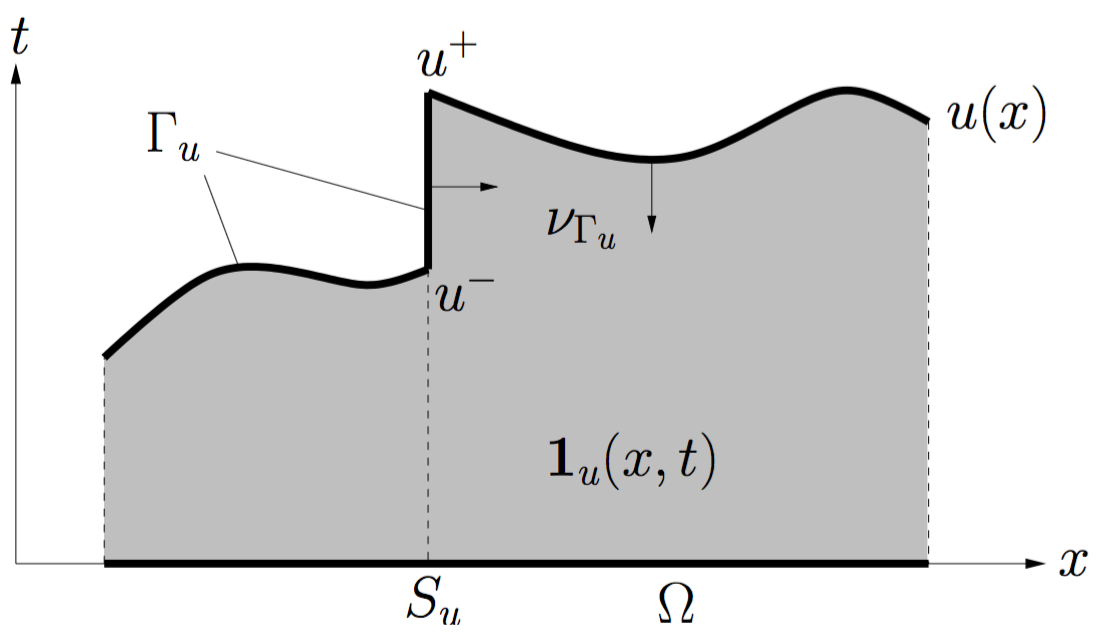
\includegraphics[width=0.8\textwidth]{img/char_func.png}
        \caption{This picture (found in \cite{Pock-et-al-iccv09}) shows the characteristic function of another function $u(x)$. The gray shaded area shows where $\mathds{1}_{u}(x, t) = 1$.}
        \label{fig:characteristic_function}
    \end{figure}

    \begin{remark}
        This lifiting method together with the following theorem assures, that the Mumford-Shah Model we are facing will be convex. As soon as we have a convex optimazation problem we can apply the primal-dual algorithm to solve it.
    \end{remark}

    Using this characteristic function, one can find in a series of paper (\cite{kelvey-sscv}, \cite{Alberti-et-al-cvpde}) a result of the convex relaxed Mumford-Shah Functional along with a proof of this result.

    \begin{theorem}[Convex Relaxation of the Mumford-Shah Functional]
    \label{convex_relaxation_of_the_mumford_shah_functional}
        For a function $u \in SBV(\Omega)$ the Mumford Shah functional can be written as
            \begin{equation}
                E(u) = \sup_{\varphi \in K} \int_{\Omega \times \mathbb{R}} \varphi D\mathds{1}_{u}, \label{eq:convex_relaxed_ms}
            \end{equation}
        with a convex set
            \begin{eqnarray}
                K = \bigg\{ \varphi \in C^{0}(\Omega \times \mathbb{R}, \mathbb{R}^{2}) &:& \varphi^{t}(x, t) \ge \frac{\varphi^{x}(x,t)^{2}}{4} - \lambda(t - f(x))^{2}, \\
                &&\bigg| \int^{t_{2}}_{t_{1}} \varphi^{x}(x,s)ds \bigg| \le \nu \bigg\}, \label{eq:set_k_continuous}
            \end{eqnarray}
        where the inequalities in the definition of $K$ hold for all $x \in \Omega$ and for all $t, t_{1}, t_{2} \in \mathbb{R}$.
    \end{theorem}

    \begin{remark}
        We used in the theorem, that we will represent a vector $\varphi \in K \subseteq \mathbb{R}^{n}$ by $\varphi(x, t) = \big( \varphi^{x}, \varphi^{t} \big)^{T}$, where $\varphi(x,t) \in \mathbb{R}^{n}$, $\varphi^{x} \in \mathbb{R}^{n-1}$ and $\varphi^{t} \in \mathbb{R}$.
    \end{remark}

    Our goal is now to minimize \ref{eq:convex_relaxed_ms} since minimizing the energy of this functional should lead to an optimal approximation $u$ of an input image $f$. Mathematically we have:

    \begin{equation}
        \min_{u \in X} E(u) = \min_{u \in X} \left( \sup_{\varphi \in K} \int_{\Omega \times \mathbb{R}} \varphi D\mathds{1}_{u} \right) \label{eq:minimize_convex_relaxed_ms}
    \end{equation}

    To compute the minimizer of this formulation we first want to substitute $\mathds{1}_{u}$ by a generic function
        \begin{equation}
            v(x, t): \Omega \times \mathbb{R} \longrightarrow [0, 1] \,\, \textnormal{which satisfies} \,\, \lim_{t \rightarrow -\infty} v(x, t) = 1, \, \, \, \lim_{t \rightarrow +\infty} v(x, t) = 0.
        \label{eq:generic_functions}
        \end{equation}
    This substitution is important to take into account, that we assume an image $u$ to be in $[0, 1]$ in this chapter. Unfortunatelly, this makes the proposed method inexact. But still, we are computing a lower bound to the global optimal solution. Further, if we only consider the characteristic function then one can show that for binary images the lower bound is indeed the global optimal value of \ref{eq:minimize_convex_relaxed_ms}. Overall, we are going to face the following, continous, convex optimization problem:
        \begin{equation}
            \min_{v \in [0, 1]} \sup_{\varphi \in K} \langle v, D\varphi \rangle = \min_{v \in [0, 1]} \sup_{\varphi \in K} \int_{\Omega \times \mathbb{R}} \varphi Dv. \label{eq:continous_saddle_point_problem}
        \end{equation}

    In the next section we will reformulate this minimization problem in the discrete setting. Additionally, we will formulate this section in the sense of the saddle-point problem \ref{eq:the_saddle_point_problem}.

% section convex_relaxation (end)

%     \section{Clarification} % (fold)
%     \label{sec:clarification}
        
%     % section clarification (end)

%     \section{A proof of convergence} % (fold)
%     \label{sec:a_proof_of_convergence}
        
%     % section a_proof_of_convergence (end)

%     \section{Minimizing the Mumford-Shah Functional} % (fold)
%     \label{sec:minimizing_the_mumford_shah_functional}
    
%     % section minimizing_the_mumford_shah_functional (end)

%         \section{Projection onto the convex sets and Dykstra's projection algorithm}

%             \subsection{Dykstra's projection algorithm} % (fold)
%             \label{sub:dykstra_s_projection_algorithm}
% %             Dykstra's algorithm finds for each r the only  \bar{x} \in C\cap D such that:

% %  \|\bar{x}-r\|^2\le \|x-r\|^2, \text{for all } x\in C \cap D, 
% % where C,D are convex sets. This problem is equivalent to finding the projection of r onto the set C\cap D, which we denote by \mathcal{P}_{C \cap D}.

%                 Consider $P$ \underline{convex} sets with $\mathbb{R}^{n} \ni X = X_{1} \cap X_{2} \cap ... \cap X_{P}$. Let $\Pi_{i}$ denote the projection onto the i-th set for $i = 1, ..., P$. And let $u_{c} \in \mathbb{R}^{n}$ be the current estimate with $u_{c} \notin X$, $u_{i}^{k} \in \mathbb{R}^{n}$ for $i = 0, ..., P$ and $v_{i}^{k} \in \mathbb{R}^{n}$ for $i = 1, ..., P$ and $k = 1, 2, ...$, where $k$ denotes the number of iterations. Then the algorithm of (Boyle and) Dykstra finds for a point $u_{c} \in \mathbb{R}^{n}$ the (only) $u^{\ast} \in X$ such that

%                 $$
%                     ||u^{\ast} - u_{c}||^{2} \le ||u - u_{c}||^{2} \,\,\, \forall u \in X.
%                 $$

%                 \begin{algorithm}\label{alg:dykstra}
%                     For $k = 1, 2, ...$ set $u^{0}_{P} = u_{c}$ and $v^{0}_{i} = 0$ for all $i = 1, ..., P$. Then iterate until convergence (e.g. $||u_{0}^{k} - u_{P}^{k}||_{2} \le \varepsilon$ with $\varepsilon$ small):

%                     \begin{eqnarray}
%                         &u_{0}^{k} = &u_{P}^{k-1}, \notag \\
%                         &\textnormal{for} \,\, &i = 1, 2, ..., P: \notag \\
%                         &&u_{i}^{k} = \Pi_{i}(u_{i-1}^{k} - v_{i}^{k-1}), \notag \\
%                         &&v_{i}^{k} = u_{i}^{k} - (u_{i-1}^{k} - v_{i}^{k-1}). \notag
%                     \end{eqnarray}
%                 \end{algorithm}

%                 \begin{proposition}
%                     The sequence $u_{0}^{k}$ in algorithm \ref{alg:dykstra} converges to the (only) point $u \in X$.
%                 \end{proposition}

%                 \begin{proof}
%                     For the proof, we refer to \cite{dykstra-et-al-aors14}.
%                     \qed
%                 \end{proof}
%             % section dykstra_s_projection_algorithm (end)

%             \subsection{Projection onto $C$}

%             One possible projection in the algorithm of Dykstra is the one onto the convex set $C$.This can be efficiently computed. To project on the set $[0, 1]$ we can easily see that this is a $l_{\infty}([0, 1])$ projection, i.e. we have:

%             % \begin{algbox}
%                 \begin{algorithm}[Clipping]
%                     To project a vector $x \in \mathbb{R}^{P \times N \times M}$ on the set
%                         \begin{equation}
%                             C = \{ x \in X: x(i,j,k) \in [0,1], \,\, x(i, j, 1) = 1, \,\, x(i, j, M) = 0 \}, \label{eq:limits}
%                         \end{equation}
%                     we have pointwise
%                         \begin{equation}
%                             x^{n+1}_{i,j,k} = \min\{1, \max \{ 0, x^{n}_{i, j, k} \} \}
%                         \end{equation}
%                     for all $i = 1, ..., P, j = 1, ..., N, k = 1, ..., M$.
%                 \end{algorithm}
%             % \end{algbox}

%             \begin{proof}
%                 Let $x^{n}_{i, j, k} \notin C$. Then let
%                 \begin{enumerate}
%                     \item $x^{n}_{i,j,k} < 0$. We have
%                     $$
%                         \underbrace{\min\{1, \underbrace{\max \{ 0, x^{n}_{i, j, k} \}}_{= 0} \}}_{= 0} \in [0, 1].
%                     $$
%                     \item $x^{n}_{i,j,k} > 1$. We have
%                     $$
%                         \underbrace{\min\{1, \underbrace{\max \{ 0, x^{n}_{i, j, k} \}}_{= x^{n}_{i, j, k}} \}}_{= 1} \in [0, 1].
%                     $$
%                 \end{enumerate}
%                 \qed
%             \end{proof}

%             % \begin{rebox}
%                 \begin{remark}
%                     By projecting onto $C$ we also need to take care about the limits in \ref{eq:limits}. For that we set $x(i, j, 1) = 1$ and $x(i, j, M) = 0$ in each projection.
%                 \end{remark}
%             % \end{rebox}

%             The projection onto the convex set $K$ is more involved since it takes into account local and non-local constraints. Therefore let us decompose the set into the sets

%             \begin{eqnarray}
%                 &K_{p}& = \bigg\{ y^{3}(i,j,k) \ge \frac{y^{1}(i,j,k)^{2} + y^{2}(i,j,k)^{2}}{4} - \lambda(\frac{k}{M} - f(i,j))^{2} \bigg\} \,\,\, \forall i, j, k \notag \\
%                 \Longleftrightarrow &K_{p}& = \bigg\{ y^{t}(i, j, k) \ge \frac{||y^{x}(i, j, k)||^{2}}{4} - \lambda(\frac{k}{M} - f(i,j))^{2} \bigg\} \,\,\, \forall i, j, k \label{eq:parabola}
%             \end{eqnarray}

%             where $y^{t}(i, j, k) = y^{3}(i, j, k)$ and $y^{x}(i, j, k) := (y^{1}(i, j, k), y^{2}(i, j, k))^{T}$. For the non-local constraint we have

%             \begin{equation}
%                 K_{nl} = \bigg\{ \left| \sum_{k_{1} \le k \le k_{2}} (y^{1}(i,j,k), y^{2}(i,j,k))^{T} \right| \le \nu \bigg\} \,\,\, \forall i, j, k_{1} \le k \le k_{2} \label{eq:nonlocal}
%             \end{equation}

%             being the non-local constraint. Then we have $K = K_{p} \cap K_{nl}$. Since $K_{p}$ is an intersection of $P \cdot N \cdot M$ set and $K_{nl}$ is an intersection of $P \cdot N \cdot (\frac{M(M-1)}{2} + M)$ sets we need an algorithm which can handle the projection of a point onto (convex) sets. First let us introduce the projections onto $K_{p}$ and $K_{nl}$.

%             \subsection{Projection onto $K_{p}$}

%                 % Since the projection onto this set also goes pointwise, we have several possibilities to compute the orthogonal projection onto a parabola.\\
%                 Since the projection onto the set $K_{p}$ is pointwise we want to drop the indices $(i, j, k)$. Note that we do not necessarily need that a $y^{x}$ is an element of $\mathbb{R}^{2}$. The following derivation holds for a larger class of problems namely having $y^{x} \in \mathbb{R}^{n}$.
%                 % To understand how a projection on a parabola can be computed we want to reformulate \ref{eq:localconst} into an optimization problem.\\
%                 \begin{describe}[]
%                     Let $\alpha > 0$, $y^{x} \in \mathbb{R}^{n}$, $y^{t} \in \mathbb{R}$ %(in our case we would have
%                     %$$
%                      %   y^{t} := y^{3}(i, j, k) + \lambda \bigg( \frac{k}{M} - f(i, j)\bigg)^{2}
%                     %$$
%                     %for all $i = 1, ..., P$, $j = 1, ..., N$, $k = 1, ..., M$) and
%                     $y = (y^{x}, y^{t})^{T} \in \mathbb{R}^{n} \times \mathbb{R}$.
%                     The projection of a $y_{0}$ with $y_{0}^{t} < \alpha ||y_{0}^{x}||_{2}^{2}$ can be written as

%                     \begin{eqnarray}
%                         &\min\limits_{y \in \mathbb{R}^{n} \times \mathbb{R}}& \frac{1}{2} ||y - y_{0}||_{2}^{2} \notag \\
%                         &\textnormal{subject to}& y^{t} \ge \alpha||y^{x}||_{2}^{2} \notag
%                     \end{eqnarray}

%                     An equivalent notation for this problem is

%                     \begin{eqnarray}
%                         &\min\limits_{y \in \mathbb{R}^{n} \times \mathbb{R}}& f(y) := \frac{(y - y_{0})^{2}}{2} \notag \\
%                         &\textnormal{subject to}& g(y) := y^{t} - \alpha ||y^{x}||_{2}^{2} \ge 0 \notag
%                     \end{eqnarray}
%                 \end{describe}

%                 To find the solution of this optimization problem we introduce some auxiliary variable (or Lagrange Multiplier) $\mu \in \mathbb{R}$ and define the Lagrangian as

%                 \begin{equation}
%                     \mathcal{L}(x, y, \mu) = f(y) - \mu g(y) = \frac{(y - y_{0})^{2}}{2} - \mu \bigg( y^{t} - \alpha||y^{x}||_{2}^{2} \bigg).
%                 \end{equation}

%                 Seeking for the local minima where $\nabla \mathcal{L}(x, y, \mu) = 0$ we even get a global minimum since our function to optimize is convex, the inequality constraint is convex and the feasible set $\mathbb{R}^{n} \times \mathbb{R}$ is also convex. We set

%                 \begin{equation}
%                     \nabla \mathcal{L}(y, \mu) =
%                     \begin{pmatrix}
%                         \partial_{y^{x}} \mathcal{L}(y, \mu) \\
%                         \partial_{y^{t}} \mathcal{L}(y, \mu) \\
%                         \partial_{\mu} \mathcal{L}(y, \mu)
%                     \end{pmatrix} = 
%                     \begin{pmatrix}
%                         y^{x} - y_{0}^{x} - \mu 2 \alpha y^{x} \\
%                         y^{t} - y_{0}^{t} - \mu \\
%                         y^{t} - \alpha||y^{x}||_{2}^{2}
%                     \end{pmatrix}
%                     = 0. \label{eq:linearSystem}
%                 \end{equation}

%                 That means, we need to solve a linear system. The first equation gives us

%                 \begin{equation}
%                     y_{0}^{x} = (\mu 2 \alpha + 1) y^{x} \Longleftrightarrow y^{x} = \frac{y_{0}^{x}}{\mu 2 \alpha + 1}, \label{eq:1stequ}
%                 \end{equation}

%                 and the second equation leads us to

%                 \begin{equation}
%                     y^{t} = y_{0}^{t} + \mu. \label{eq:2ndequ}
%                 \end{equation}

%                 At this point we can solve this system in two ways - if $y_{0}^{t} \ge \alpha ||y_{0}^{x}||_{2}^{2}$ is not true already
%                 \begin{enumerate}
%                     \item By plugging these two equalities into the third equation, we get

%                 \begin{eqnarray}
%                     y_{0}^{t} + \mu - \alpha \bigg|\bigg|\frac{y_{0}^{x}}{\mu 2 \alpha + 1}\bigg|\bigg|_{2}^{2} = 0 &\Longleftrightarrow& y_{0}^{t} + \mu - \frac{\alpha}{(\mu 2 \alpha + 1)^{2}} ||y_{0}^{x}||_{2}^{2} = 0 \notag \\
%                     &\Longleftrightarrow& (\mu 2 \alpha + 1)^{2} y_{0}^{t} + (\mu 2 \alpha + 1)^{2} \mu - \alpha ||y_{0}^{x}||_{2}^{2} = 0 \notag \\
%                     &\Longleftrightarrow& (4 \mu^{2} \alpha^{2} + 4 \mu \alpha + 1) y_{0}^{t} + 4 \mu^{3} \alpha^{2} + 4 \mu^{2} \alpha + \mu - \alpha ||y_{0}^{x}||_{2}^{2} = 0 \notag \\
%                     &\Longleftrightarrow& 4 \alpha^{2} \mu^{3} + \mu^{2} (4 \alpha^{2} y_{0}^{t} + 4 \alpha) + \mu (4 \alpha y_{0}^{t} + 1) + y_{0}^{t} - \alpha ||y_{0}^{x}||_{2}^{2} = 0. \notag
%                 \end{eqnarray}

%                 Solving this equation is straightforward since computing the zeroes can be done by Newton's algorithm with

%                 \begin{equation}
%                     \mu^{k+1} = \mu^{k} - \frac{h(\mu)}{h^{'}(\mu)}, \label{eq:newton}
%                 \end{equation}

%                 for $k = 1, 2, ...$.

%                 If we set
%                 $$
%                     h(\mu) = 4 \alpha^{2} \mu^{3} + \mu^{2} (4 \alpha^{2} y_{0}^{t} + 4 \alpha) + \mu(4 \alpha y_{0}^{t} + 1) + y_{0}^{t} - \alpha ||y_{0}^{x}||_{2}^{2},
%                 $$
%                 we observe
%                 $$
%                     h^{'}(\mu) = 12 \alpha^{2} \mu^{2} + 2 \mu (4 \alpha^{2} y_{0}^{t} + 4 \alpha) + (4 \alpha y_{0}^{t} + 1).
%                 $$
%                 At the end we are having the update of a $\mu^{k+1}$ with
%                 \begin{equation}
%                     \mu^{k+1} = \mu^{k} - \frac{4 \alpha^{2} \mu^{3} + \mu^{2} (4 \alpha^{2} y_{0}^{t} + 4 \alpha) + \mu(4 \alpha y_{0}^{t} + 1) + y_{0}^{t} - \alpha ||y_{0}^{x}||_{2}^{2}}{12 \alpha^{2} \mu^{2} + 2 \mu (4 \alpha^{2} y_{0}^{t} + 4 \alpha) + (4 \alpha y_{0}^{t} + 1)}.
%                 \end{equation}
%                 In \cite{Chambolle-et-al-10} they suggest setting $\mu^{0} = \max \{ 0, - \frac{2 y_{0}^{t}}{3} \}$. The algorithm converges within 10-20 iterations to a quite accurate solution.\\
%                 The projected vector $y$ of our problem is then given by
%                 \begin{equation}
%                     y = \bigg( \frac{y_{0}^{x}}{\mu 2 \alpha + 1}, y_{0}^{t} + \mu \bigg). \label{eq:newtonSolution}
%                 \end{equation}

%                 \item For the second approach we note that \ref{eq:1stequ} and \ref{eq:2ndequ} hold and the third equation in \ref{eq:linearSystem} can only hold if
%                 \begin{equation}
%                     y^{t} = \alpha ||y^{x}||_{2}^{2} \Longleftrightarrow \alpha ||y^{x}||_{2}^{2} = y_{0}^{t} + \mu. \label{eq:tmp1}
%                 \end{equation}
%                 With \ref{eq:1stequ} we can also compute the solution of $\mu$ by noticing that

%                 \begin{eqnarray}
%                     ||y^{x}||_{2} = \bigg|\bigg| \frac{y_{0}^{x}}{1 + 2 \alpha \mu} \bigg|\bigg|_{2} &\Longleftrightarrow& ||y^{x}||_{2} = \frac{1}{1 + 2 \alpha \mu} ||y_{0}^{x}||_{2} \notag \\
%                     &\Longleftrightarrow& \frac{1}{1 + 2 \alpha \mu} = \frac{||y^{x}||_{2}}{||y_{0}^{x}||_{2}} \notag \\
%                     &\Longleftrightarrow& 2 \alpha \mu = \frac{||y_{0}^{x}||_{2}}{||y^{x}||_{2}} - 1 \notag \\
%                     &\Longleftrightarrow& \mu = \frac{1}{2 \alpha} \bigg( \frac{||y_{0}^{x}||_{2}}{||y^{x}||_{2}} \bigg). \notag
%                 \end{eqnarray}

%                 Using the solution of $\mu$ in \ref{eq:tmp1} we get

%                 \begin{eqnarray}
%                     \alpha ||y^{x}||_{2}^{2} = y_{0}^{t} + \frac{1}{2 \alpha} \bigg( \frac{||y_{0}^{x}||_{2}}{||y^{x}||_{2}} \bigg) &\overbrace{\Longleftrightarrow}^{\cdot 2 \alpha ||y^{x}||_{2}}& 2 \alpha^{2} ||y^{x}||_{2}^{3} = 2 \alpha ||y^{x}||_{2} y_{0}^{t} + ||y_{0}^{x}||_{2} - 1 \notag \\
%                     &\Longleftrightarrow& 2 \alpha^{2} ||y^{x}||_{2}^{3} + (1 - 2 \alpha y_{0}^{t}) ||y^{x}||_{2} - ||y_{0}^{x}||_{2} = 0. \notag \\ 
%                     &\overbrace{\Longleftrightarrow}^{\cdot 4 \alpha}& 8 \alpha^{3} ||y^{x}||_{2}^{3} + 4 \alpha (1 - 2 \alpha y_{0}^{t}) ||y^{x}||_{2} - 4 \alpha ||y_{0}^{x}||_{2} = 0. \notag \\
%                     &\Longleftrightarrow& (2 \alpha ||y^{x}||_{2})^{3} + 2 (1 - 2 \alpha y_{0}^{t}) 2 \alpha ||y^{x}||_{2} - 4 \alpha ||y_{0}^{x}||_{2} = 0. \notag \\
%                     &\Longleftrightarrow& t^{3} + 3bt - 2a = 0, \label{eq:cubic}
%                 \end{eqnarray}

%                 with $a = 2 \alpha ||y_{0}^{x}||_{2}$, $b = \frac{2}{3}(1 - 2 \alpha y_{0}^{t})$ and $t = 2 \alpha ||y^{x}||_{2}$.\\
%                 The cubic equation \ref{eq:cubic} in $t$ can efficiently be solved using \cite{kelvey-ajp}.

%                 \end{enumerate}

%                 The result of the work mentioned is summarized in the following algorithm. Notice that we already computed the factors $a$ and $b$. The others follow through the proof.

%                 % After computing the optimal $\mu$ we get the solution to our optimization problem by plugging the Lagrange Multiplier into \ref{eq:1stequ} and \ref{eq:2ndequ} and computing $y^{x}, y^{t}$ respectively.

%                 % \begin{enumerate}
%                 %     \item Using Lagrange-Multipliers to rewrite the minimization problem and then applying Newton's method.
%                 %     \item Following a straightforward formulation proposed in (Evgeny).
%                 % \end{enumerate}

%                 % We want to start with the method proposed in (Evgeny).

%                     \begin{algorithm}
%                         % Let $\alpha > 0$. For $y_{0}^{x} \in \mathbb{R}^{n}$ and $y_{0} \in \mathbb{R}$ the projection onto the parabola of the form

%                         % \begin{equation}
%                         %     \arg \min_{x \in \mathbb{R}^{n}, y \in \mathbb{R}, y \ge \alpha ||x||_{2}^{2}} \frac{(x - y_{0}^{x})^{2}}{2} + \frac{(y - y_{0})^{2}}{2}.
%                         % \end{equation}

%                         If already $y_{0}^{t} \ge \alpha ||y_{0}^{x}||_{2}^{2}$, the solution is $(y^{x}, y^{t}) = (y_{0}^{x}, y_{0}^{t})$. Otherwise, with $a := 2 \alpha ||y_{0}^{x}||_{2}$, $b := \frac{2}{3} (1 - 2 \alpha y_{0}^{t})$, and

%                             \[
%                                 d =
%                                     \begin{dcases*}
%                                         a^{2} + b^{3} & \textnormal{if $b \ge 0$}\\
%                                         (a - \sqrt{-b}^{3})(a + \sqrt{-b}^{3}) & \textnormal{else}
%                                     \end{dcases*}
%                             \]

%                         set

%                             \[
%                                 v =
%                                     \begin{dcases*}
%                                         c - \frac{b}{c} \,\, \textnormal{with} \,\, c = \sqrt[3]{a + \sqrt{d}} & \textnormal{if $d \ge 0$}\\
%                                         2 \sqrt{-b} \cos \bigg( \frac{1}{3} \arccos \frac{a}{\sqrt{-b}^{3}} \bigg) & \textnormal{else}.
%                                     \end{dcases*}
%                             \]

%                         If $c = 0$ in the first case, set $v := 0$. The solution is then given by

%                             \[
%                                 y^{x} =
%                                     \begin{dcases*}
%                                         \frac{v}{2\alpha} \frac{y_{0}^{x}}{||y_{0}^{x}||_{2}} & \textnormal{if $y_{0}^{x} \ne 0$}\\
%                                         0 & \textnormal{else}
%                                     \end{dcases*}
%                             \]

%                         and $y^{t} = \alpha ||y^{x}||_{2}^{2}$.
%                     \end{algorithm}

%                     % \begin{proof}
%                     %     Later...
%                     % \end{proof}

%                 The above method states that the projection onto the parabola can be done by one cycle of straightforward computations. The implementation of it is quite simple and computation time is fast.% But as mentioned there is another approach for this projection.\\

%             \subsection{Projection onto $K_{nl}$}

%                 This set is a combination of non-local constraints, meaning that in a fixed point $(i, j, k)$ you sum up for all $k_{1} \le k \le k_{2}$. For that reason you can not project pointwise. First of all we want to present the algorithm:

%                 % Let $y_{k} := (y^{1}(i, j, k), y^{2}(i, j, k))^{T}$. Then the projection $y = (y_{1}, ..., y_{M})^{T}$ of a $y_{0} = (y_{0}_{1}, ..., y_{0}_{M})^{T}$ is - for each combination $k_{1} \le k \le k_{2}$ - of the following problem:
%                 % \begin{algbox}
%                     \begin{algorithm}[Soft Shrinkage Scheme]\label{alg:softshrinkage}
%                         Let $y^{i}_{k} := (y^{1}(i, j, k), y^{2}(i, j, k))^{T} \in \mathbb{R}^{2}$, $y^{i} := (y^{i}_{1}, ..., y^{i}_{M})^{T} \in \mathbb{R}^{2 \times M}$ for all $i = 1, 2, ...$. Then the projection $y^{n+1}$ of a $y^{n}$ - for an arbitrary, fixed pair $(k_{1}, k_{2})$ with $1 \le k_{1} \le k \le k_{2} \le M$ - is computed by:

%                             \[
%                                 y^{n+1} =
%                                     \begin{dcases*}
%                                         y^{n} + \frac{s - \tilde{s}}{k_{2} - k_{1} + 1} & \textnormal{if $k_{1} \le k \le k_{2}$}, \\
%                                         y^{n} & \textnormal{else},
%                                     \end{dcases*}
%                             \]

%                         where $s \in \mathbb{R}^{2}, \tilde{s} \in \mathbb{R}^{2}$ with

%                             $$\tilde{s} = \sum_{k_{1} \le k \le k_{2}} y_{k}$$

%                         and

%                             \[
%                                 s =
%                                     \begin{dcases*}
%                                         \tilde{s} & \textnormal{if $||\tilde{s}||_{2} \le \nu$},\\
%                                         \Pi_{||\cdot||_{2} \le \nu}(\tilde{s}) = \frac{\nu}{||\tilde{s}||_{2}} \tilde{s} & \textnormal{else}.
%                                     \end{dcases*}
%                             \]

%                         % \begin{equation}
%                         %     \min\limits_{y_{k} \in \mathbb{R}^{2}} \frac{1}{2} \sum_{k = 1}^{M} ||y_{k} - \tilde{y}_{k}||^{2} \,\,\, \textnormal{s.t.} \,\,\, \bigg{|} \bigg{|} \sum_{k_{1} \le k \le k_{2}} (y^{1}(i, j, k), y^{2}(i, j, k))^{T} \bigg{|} \bigg{|}_{2} \le \nu. \label{eq:minnonlocal}
%                         % \end{equation}
%                         % It follows that we have $y_{k} = \tilde{y}_{k}$ for all $k < k_{1}$ and $k > k_{2}$.\\
%                         % If $k_{1} \le k \le k_{2}$ one can show that we have:
%                         % \begin{equation}
%                         %     y_{k} = \tilde{y}_{k} + \frac{s - s_{0}}{k_{2} - k_{1} + 1},
%                         % \end{equation}
%                         % where
%                         % $$s_{0} = \sum_{k_{1} \le k \le k_{2}} \tilde{y}_{k}$$
%                         % and
%                         % $$s = \Pi_{||\cdot||_{l^{2}} \le \nu} (s_{0}).$$
%                     \end{algorithm}
%                 % \end{algbox}

%                 Since this procedure needs a clarification, we want to introduce the KKT conditions.

%                 % \begin{defbox}
%                     \begin{theorem}[Karush-Kuhn-Tucker Optimality Conditions]
%                         Consider the optimization problem
%                         \begin{eqnarray}
%                             \min_{x \in \mathbb{R}^{n}} &&f(x) \notag \\
%                             \textnormal{s.t.} \,\, && g_{i}(x) \le 0, i = 1, ..., m \notag
%                         \end{eqnarray}

%                         Defining the Lagrangian function to this optimization problem we have

%                         \begin{equation}
%                             \mathcal{L}(x, \lambda) = f(x) + \lambda, g(x),
%                         \end{equation}

%                         with $\lambda \in \mathbb{R}^{m}$ are called the Lagrange-Multipliers.\\

%                         Then if the objective function $f: \mathbb{R}^{n} \longrightarrow \mathbb{R}$ and the constraint functions $g_{i}: \mathbb{R} \longrightarrow \mathbb{R}$ are continously differentiable at a point $x^{*}$ then it holds:\\
%                         $$x^{*} \, \textnormal{is a local minimum} \, \Longleftrightarrow \, \textnormal{there exists a unique} \, \lambda^{*} \, \textnormal{such that}$$
%                         \begin{itemize}
%                             \item Stationarity:
%                             $$\nabla_{x} \mathcal{L}(x^{*}, \lambda^{*}) = 0$$
%                             \item Complementary Slackness:
%                             $$\lambda^{*}_{i} g(x^{*}) = 0 \, \, \, \forall i = 1, ..., m$$
%                             \item Primal Feasibility:
%                             $$g_{i}(x^{*}) \le 0 \, \, \, \forall i = 1, ..., m$$
%                             \item Dual Feasibility:
%                             $$\lambda^{*}_{i} \ge 0 \, \, \, \forall i = 1, ..., m$$
%                         \end{itemize}
%                     \end{theorem}
%                 % \end{defbox}

%             \begin{proof}[Proof of Algorithm \ref{alg:softshrinkage}]
%                 Let $y_{k}, \tilde{y}_{k} \in \mathbb{R}^{2}$ and $y, \tilde{y} \in \mathbb{R}^{2 \times M}$ have the same form as in \ref{alg:softshrinkage}. Then for a fixed pair $(k_{1}, k_{2})$ we face the following optimization problem: %$K = k_{2} - k_{1} + 1$, $m = \frac{M(M-1)}{2}$, 
%                 % $y_{k} \in \mathbb{R}^{2}$, $\tilde{y}_{k} \in \mathbb{R}^{2}$, $y = (y_{1}, ..., y_{M})^{T} \in \mathbb{R}^{2 \times M}$ and $\tilde{y} = (\tilde{y}_{1}, ..., \tilde{y}_{M})^{T} \in \mathbb{R}^{2 \times M}$. Then for a fixed pair $(k_{1}, k_{2})$ we have% have that \ref{eq:minnonlocal} is equivalent to

%                 \begin{eqnarray}
%                     &\min\limits_{y \in \mathbb{R}^{2 \times M}}& \frac{1}{2} ||y - \tilde{y}||^{2}_{2} \notag \\
%                     &\textnormal{subject to}& \bigg{|} \bigg{|} \sum_{k_{1} \le k \le k_{2}} y_{k} \bigg{|} \bigg{|}_{2} \le \nu. \notag
%                 \end{eqnarray}

%                 This equivalent to

%                 \begin{eqnarray}
%                     &\min\limits_{y \in \mathbb{R}^{2 \times M}}& f(y) \notag \\
%                     &\textnormal{subject to}& g(y) \le 0, \label{eq:inequalityConstraint}
%                 \end{eqnarray}

%                 if we set
%                     $$f(y) = \sum_{k = 1}^{M} \frac{(y_{k} - \tilde{y}_{k})^{2}}{2}$$
%                 and
%                     $$g(y) = \frac{1}{2} \bigg{|} \bigg{|} \sum_{k_{1} \le k \le k_{2}} y_{k} \bigg{|} \bigg{|}_{2}^{2} - \frac{1}{2} \nu^{2}.$$

%                 This problem states that we try to find the closest $y$ to $\tilde{y}$ whose components fullfil the inequality constraint in \ref{eq:inequalityConstraint}.\\

%                 % \begin{equation}
%                 %     \min\limits_{y_{k} \in \mathbb{R}^{2}} \frac{1}{2} \sum_{k = 1}^{M} ||y_{k} - \tilde{y}_{k}||^{2} \,\,\, \textnormal{s.t.} \,\,\, \frac{1}{2} \bigg{|} \bigg{|} \sum_{k_{1} \le k \le k_{2}} (y^{1}(i, j, k), y^{2}(i, j, k))^{T} \bigg{|} \bigg{|}_{2}^{2} - \frac{1}{2} \nu^{2} \le 0 \notag
%                 % \end{equation}

%                 Let us now introduce a new variable $\lambda \in \mathbb{R}$ which is called Lagrange Multiplier and observe the Lagrange function (or Lagrangian) with

%                 % \begin{equation}
%                 %     \min_{y \in \mathbb{R}^{2 \times M}} f(y) \,\,\, \textnormal{s.t.} \,\,\, g_{i}(y) \le \nu \,\,\, \forall i = 1, ..., m \notag
%                 % \end{equation}

%                 % has the following form

%                 \begin{equation}
%                     \mathcal{L}(y, \lambda) = f(y) + \lambda g(y)% = \frac{1}{2} \sum_{k = 1}^{M} ||y_{k} - \tilde{y}_{k}||^{2} + \sum_{l = 1}^{K} \lambda_{l} g_{l}(y),
%                 \end{equation}

%                 Looking at \underline{Stationarity} condition to find a valid $\lambda^{\ast}$ and $y^{\ast}$ leads us to:

%                 \begin{equation}
%                     \nabla_{y} \mathcal{L}(y^{\ast}, \lambda^{\ast}) = \nabla_{y} f(y^{\ast}) + \lambda \nabla_{y} g(y^{\ast}) =
%                     \underbrace{\begin{pmatrix}
%                         y^{\ast}_{1} - \tilde{y}_{1} \\
%                          \\
%                         \vdots \\
%                          \\
%                         y^{\ast}_{M} - \tilde{y}_{M}
%                     \end{pmatrix}}_{\in \mathbb{R}^{M}}
%                     + \lambda^{\ast}
%                     \underbrace{\begin{pmatrix}
%                         0 \\
%                         \vdots \\
%                         0 \\
%                         \sum\limits_{k_{1} \le k \le k_{2}} y^{\ast}_{k} \\
%                         \vdots \\
%                         \sum\limits_{k_{1} \le k \le k_{2}} y^{\ast}_{k} \\
%                         0 \\
%                         \vdots \\
%                         0
%                     \end{pmatrix}}_{\in \mathbb{R}^{M}}
%                     = 0,
%                 \end{equation}

%                 where the zeroes in the last vector are obtain for all components where $k < k_{1}$ and $k > k_{2}$. In these lines we already see that we get

%                     $$y^{\ast}_{k} = \tilde{y}_{k} \,\,\, \textnormal{if} \,\, k < k_{1} \,\, \textnormal{and} \,\, k > k_{2}.$$

%                 Let us now take a closer look at the i-th line where $\nabla_{y_{k}} g(y) \ne 0$. Then we have

%                     \begin{equation}
%                         y^{\ast}_{i} - \tilde{y}_{i} + \lambda^{\ast} \sum_{k_{1} \le k \le k_{2}} y^{\ast}_{k} = 0. \label{eq:ithRow}
%                     \end{equation}

%                 We set % state that the optimal $\lambda^{\ast}$ is of the form

%                 %     \begin{equation}
%                 %         \lambda^{\ast} = \frac{1}{k_{2} - k_{1} + 1} \bigg( \frac{\nu}{||\tilde{s}||_{2}} - 1 \bigg). \label{eq:lambda}
%                 %         % \lambda^{\ast} = \frac{\nu}{||\sum\limits_{k_{1} \le k \le k_{2}} y^{\ast}||_{2}} - 1. \label{eq:lambda}
%                 %     \end{equation}

%                 % with

%                     $$\tilde{s} := \sum\limits_{k_{1} \le k \le k_{2}} \tilde{y}_{k}$$

%                 and define a $s \in \mathbb{R}^{2}$ as

%                     \[
%                         s =
%                             \begin{dcases*}
%                                 \tilde{s} & \textnormal{if $||\tilde{s}||_{2} \le \nu$},\\
%                                 \Pi_{||\cdot||_{2} \le \nu}(\tilde{s}) = \frac{\nu}{||\tilde{s}||_{2}} \tilde{s} & \textnormal{else}.
%                             \end{dcases*}
%                     \]

%                 \newpage

%                 For finding the optimal values $y^{\ast}_{k}$ we want to distinguish between two cases:

%                 \begin{enumerate}
%                     \item $||\sum\limits_{k_{1} \le k \le k_{2}} \tilde{y}_{k}||_{2} \le \nu$:\\
%                     Setting $y^{\ast}_{k} = \tilde{y}_{k} + \frac{s - \tilde{s}}{k_{2} - k_{1} + 1} = \tilde{y}_{k}$ for all $k_{1} \le k \le k_{2}$ and $s = \tilde{s}$ leads to
%                         \begin{equation}
%                             \frac{1}{2} ||\sum_{k_{1} \le k \le k_{2}} y^{\ast}_{k}||_{2}^{2} - \frac{1}{2} \nu^{2} \le 0, \label{eq:caseOne}
%                         \end{equation}
%                     % which validates the \underline{Primal Feasibility} condition.
%                     It follows for the \underline{Complementary Slackness} condition that we can choose an arbitrary $\lambda^{\ast} \ge 0$ if we have equality in \ref{eq:caseOne} and $\lambda^{\ast} = 0$ else to derive the \underline{Dual Feasibility} condition. We set
%                     % The \underline{Complementary Slackness} condition claims that in this case% validates the \underline{Dual Feasibility} condition in this case because having equality in \ref{eq:caseOne} leads to
%                         $$\lambda^{\ast} = 0.$$

%                     % since $||\tilde{s}||_{2} \le \nu$.
%                     % which is equivalent to
%                         % ||\tilde{s}||_{2} = ||\sum\limits_{k_{1} \le k \le k_{2}} \tilde{y}^{k}||_{2} = 
%                         % $$\frac{\nu}{||\tilde{s}||_{2}} - 1 = 0 \Longleftrightarrow ||\tilde{s}||_{2} = \nu.$$
%                     % On the other hand if the inequality holds we have
%                     %     % ||\tilde{s}||_{2} = ||\sum\limits_{k_{1} \le k \le k_{2}} \tilde{y}^{k}||_{2} = 
%                     %     $$||\sum\limits_{k_{1} \le k \le k_{2}} y^{\ast}_{k}||_{2} < \nu \Longrightarrow \lambda^{\ast} = \underbrace{\frac{\nu}{||\sum\limits_{k_{1} \le k \le k_{2}} y^{\ast}_{k}||_{2}}}_{> 1} - 1 > 0.$$
%                     % Then $\lambda^{\ast}$ additionally satisfies the \underline{Complementary Slackness} condition.
%                     \item $||\sum\limits_{k_{1} \le k \le k_{2}} \tilde{y}_{k}||_{2} > \nu$:\\
%                     % If the equality holds we know that $s(\tilde{s})$
%                     Here, we would violate the \underline{Primal Feasibility} condition if we set $y^{\ast}_{k} = \tilde{y}_{k}$ for all $k_{1} \le k \le k_{2}$. For this reason we choose
%                         $$y^{\ast}_{k} = \tilde{y}_{k} + \frac{s - \tilde{s}}{k_{2} - k_{1} + 1} \,\,\,\,\,\, \forall k_{1} \le k \le k_{2}$$
%                         % $$y^{\ast}_{k} = \frac{\nu}{||\tilde{s}||_{2}} \tilde{y}_{k} \,\,\,\,\,\, \forall k_{1} \le k \le k_{2}$$
%                     We observe for the \underline{Primal Feasibility} condition that
%                         \begin{eqnarray}
%                             \frac{1}{2} ||\sum_{k_{1} \le k \le k_{2}} y^{\ast}_{k}||_{2}^{2} - \frac{1}{2} \nu^{2} &=& \label{eq:caseTwo} \\
%                             &=& \frac{1}{2(k_{2} - k_{1} + 1)} ||\sum_{k_{1} \le k \le k_{2}} \tilde{y}_{k} + (s - \tilde{s})||_{2}^{2} - \frac{1}{2} \nu^{2}\notag \\
%                             &=& \frac{1}{2} ||\sum_{k_{1} \le k \le k_{2}} \tilde{s} + s - \tilde{s}||_{2}^{2} - \frac{1}{2} \nu^{2} = \frac{1}{2} \underbrace{||s||_{2}^{2}}_{= \nu^{2}} - \frac{1}{2} \nu^{2} = 0. \notag
%                         \end{eqnarray}
%                     Using this equality we already see that \underline{Complementary Slackness} is fullfild with a \underline{dual feasible} $\lambda^{\ast} \ge 0$. Since we set $y^{\ast}_{k} = \tilde{y}_{k} + \frac{s - \tilde{s}}{k_{2} - k_{1} + 1}$ we can plug $y^{\ast}$ into \ref{eq:ithRow} to derive $\lambda^{\ast}$. It follows %We still need to proof that \ref{eq:lambda} is valid with this choice of $y^{\ast}_{k}$.

%                         \begin{eqnarray}
%                             &&y^{\ast}_{i} - \tilde{y}_{i} + \frac{\lambda^{\ast}}{k_{2} - k_{1} + 1} \sum_{k_{1} \le k \le k_{2}} y^{\ast}_{k} = \notag \\
%                             &=& \tilde{y}_{i} + \frac{s - \tilde{s}}{k_{2} - k_{1} + 1} - \tilde{y}_{i} + \frac{\lambda^{\ast}}{k_{2} - k_{1} + 1} \sum_{k_{1} \le k \le k_{2}} \tilde{y}_{k} + \frac{s - \tilde{s}}{k_{2} - k_{1} + 1} \notag \\
%                             &=& \frac{s - \tilde{s}}{k_{2} - k_{1} + 1} + \frac{\lambda^{\ast}}{k_{2} - k_{1} + 1} \bigg( \underbrace{\sum_{k_{1} \le k \le k_{2}} \tilde{y}_{k}}_{= \tilde{s}} + \underbrace{\sum_{k_{1} \le k \le k_{2}} \frac{s - \tilde{s}}{k_{2} - k_{1} + 1}}_{= \frac{(k_{2} - k_{1} + 1) (s - \tilde{s})}{k_{2} - k_{1} + 1} = s - \tilde{s}} \bigg) \notag \\
%                             &=& \frac{s - \tilde{s}}{k_{2} - k_{1} + 1} + \frac{\lambda^{\ast}}{k_{2} - k_{1} + 1} (\tilde{s} + s - \tilde{s}) \notag \\
%                             &=& \frac{s - \tilde{s}}{k_{2} - k_{1} + 1} + \frac{\lambda^{\ast}}{k_{2} - k_{1} + 1}s \notag \\
%                             &=& \frac{1}{k_{2} - k_{1} + 1} (s - \tilde{s} + \lambda^{\ast}s) = 0 \label{eq:equalsZero}
%                         \end{eqnarray}

%                     Now we can solve for $\lambda^{\ast}$ using that the last equation \ref{eq:equalsZero} is equivalent to

%                         \begin{eqnarray}
%                             (s - \tilde{s} + \lambda^{\ast} s) = 0 &\overbrace{\Longleftrightarrow}^{||\tilde{s}||_{2} > \nu}& \bigg(\frac{\nu}{||\tilde{s}||_{2}}\tilde{s} - \tilde{s} + \lambda^{\ast} \frac{\nu}{||\tilde{s}||_{2}}\tilde{s} \bigg) = 0 \notag \\
%                             &\Longleftrightarrow& \tilde{s} \bigg( \frac{\nu}{||\tilde{s}||_{2}} - 1 + \lambda^{\ast} \frac{\nu}{||\tilde{s}||_{2}} \bigg) = 0 \notag \\
%                             &\Longleftrightarrow& \frac{\nu}{||\tilde{s}||_{2}} - 1 + \lambda^{\ast} \frac{\nu}{||\tilde{s}||_{2}} = 0 \notag \\
%                             &\Longleftrightarrow& \lambda^{\ast} \frac{\nu}{||\tilde{s}||_{2}} = 1 - \frac{\nu}{||\tilde{s}||_{2}} \notag \\
%                             &\Longleftrightarrow& \lambda^{\ast} = \underbrace{\frac{||\tilde{s}||_{2}}{\nu}}_{> 1} - 1 > 0. \notag
%                         \end{eqnarray}

%                     This satisfies the \underline{Dual Feasibility} condition.

%                         % $$||\tilde{s}||_{2} = ||\sum\limits_{k_{1} \le k \le k_{2}} \tilde{y}_{k}||_{2} = ||\sum\limits_{k_{1} \le k \le k_{2}} \frac{||\tilde{s}||_{2}}{\nu} y^{\ast}||_{2} = ||\tilde{s}||_{2} =  \nu \Longrightarrow \lambda^{\ast} = 1 - 1 = 0.$$

%                         % $$\nu = ||\sum\limits_{k_{1} \le k \le k_{2}} y^{\ast}_{k}||_{2} = ||\frac{\nu}{||\tilde{s}||_{2}} \sum\limits_{k_{1} \le k \le k_{2}} \tilde{y}^{k}||_{2} = ||\tilde{s}||_{2} =  \nu \Longrightarrow \lambda^{\ast} = 1 - 1 = 0.$$

%                         % \begin{equation}
%                         %     y^{\ast}_{i} - \tilde{y}_{i} + \frac{\lambda^{\ast}}{k_{2} - k_{1} + 1} \tilde{s} = \frac{\nu}{||\tilde{s}||_{2}} \tilde{y}_{i} - \tilde{y}_{i} + \frac{1}{k_{2} - k_{1} + 1} \bigg( \frac{\nu}{||\tilde{s}||_{2}} - 1 \bigg) \tilde{s}
%                         % \end{equation}
%                     % First, we define a two-dimensional vector $s$ with
%                     %     \begin{equation}
%                     %         s(p) = \Pi_{||\cdot||_{2} \le \nu} (p) = \frac{\nu}{||p||_{2}} p.
%                     %     \end{equation}
%                     % If the equality in \ref{eq:caseTwo} holds. Then $||$
%                 \end{enumerate}

%                 With the choices of $\tilde{s}, s$ and

%                     $$y^{\ast}_{k} = \tilde{y}_{k} + \frac{s - \tilde{s}}{k_{2} - k_{1} + 1} \,\,\,\,\,\, \forall k_{1} \le k \le k_{2}$$

%                 we solved \ref{eq:ithRow} (\underline{Stationarity}). Applying this procedure to each combination of the $(k_{1}, k_{2})$ and replacing $y^{\ast}$ by $y^{n+1}$, $\tilde{y}$ by $y^{n}$ respectively, we observe our algorithm.
%                 \qed
%             \end{proof}

%                 % with $\lambda \in \mathbb{R}^{m}$ and $\lambda_{i} \ge 0$ for all $i = 1, ..., m$.
%                 % With this and the fact that the inequality constraint also holds for all $i = 1, ..., m$ the \underline{Primal} and the \underline{Dual Feasibility} are already fullfild.\\ 

%                 % Applying \underline{Stationarity} condition we have:

%                 % \begin{equation}
%                 %     \nabla \mathcal{L}(x^{*}, \lambda^{*}) = 0 \Longleftrightarrow - \nabla f(y^{*}) = \sum_{l = 1}^{m} \lambda^{*}_{l} \nabla g_{l}(y^{*}).
%                 % \end{equation}

%                 % And \underline{Complementary Slackness} telling us that

%                 % \begin{equation}
%                 %     \lambda^{*} g(y^{*}) = 0.% \bigg( \frac{1}{2} \bigg{|} \bigg{|} \sum_{k_{1} \le k \le k_{2}} (y^{1}(i, j, k), y^{2}(i, j, k))^{T} \bigg{|} \bigg{|}_{2}^{2} - \frac{1}{2} \nu^{2} \bigg) = 0.
%                 % \end{equation}

%         % Back to the convex set $K$ we find that this set is the intersection of several sets. In \ref{eq:localconst} you find local constraints, more precisely parabola constraints. This constraint is pixel wise. If the third component of a vector $y$ namely $y^{3}$ satisfies this inequality the vector $y$ already lies in the constraint set \ref{eq:localconst}. If not some computations need to be done. We'll come back to that later. \\
%         % On the other hand the set in \ref{eq:nonlocalconst} is more complicated and also needs special treatment. This set takes not only values from one fixed voxel into account but sums up several voxel from a range $k_{1}$ to $k_{2}$. In the end we need to have that $y \in K$ and $y$ must satisfy both constraints. \\

%         \section{An alternative approach using Lagrange Multiplier}
%             Let $f(x, y) := \langle Ax, y \rangle$. Hence we have
%                 \begin{equation}
%                     \min_{x \in C} \max_{y \in K} f(x, y) = \min_{x \in C} \max_{y \in K} \langle Ax, y \rangle. \label{eq:original}
%                 \end{equation}
%             Rewrite non-local-constraint in the set $K$ - \ref{eq:localconst} is pointwise so this is already easy to compute: \\
%             We get the formulation
%                 \begin{equation}
%                     ||p_{k_{1}, k_{2}}||_{2} \le \nu \,\,  \textnormal{ s.t. } \, \, p_{k_{1}, k_{2}} = \sum_{k_{1} \le k \le k_{2}} (y_{1}(i, j, k), y_{2}(i, j, k))^{T} \label{eq:lmnew}
%                 \end{equation}
%             which corresponds to \ref{eq:nonlocalconst}. \\
%             The constraint functions in \ref{eq:lmnew} is equivalent to
%                 \begin{equation}
%                     g(p, y) := p_{k_{1}, k_{2}} - \sum_{k_{1} \le k \le k_{2}} (y_{1}(i, j, k), y_{2}(i, j, k))^{T} = 0 \label{eq:gofp}
%                 \end{equation}
%             holding for all combinations of $k_{1}, k_{2}$ with $1 \le k_{1} \le k \le k_{2} \le M$. \\
%             Let $K = \frac{M(M-1)}{2}$ be all possible combinations of the $k_{1}, k_{2}$. For a Lagrange (dual) function $\mathcal{L}$ depending on the optimization problem in \ref{eq:original} we get
%                 \begin{eqnarray}
%                     \mathcal{L}(x, y, \lambda, p) &=& f(x, y) + \sum_{K} \lambda_{K} g(p, y) = \notag \\
%                     &&\langle Ax, y \rangle + \sum_{k_{1} = 1}^{M} \sum_{k_{2} = k_{1}}^{M} \langle \lambda_{k_{1}, k_{2}}, p_{k_{1}, k_{2}} - \sum_{k_{1} \le k \le k_{2}} (y_{1}(i, j, k), y_{2}(i, j, k))^{T} \rangle.
%                 \end{eqnarray}
%             where $x = x(i, j, k) \in \mathbb{R}^{N \times N \times M}, y(i, j, k) = (y_{1}(i, j, k), y_{2}(i, j, k), y_{3}(i, j, k))^{T} \in \mathbb{R}^{3 \times N \times N \times M}, \lambda(i, j, k) \in \mathbb{R}^{2 \times K \times N \times N}$ and $p(i, j, k) \in \mathbb{R}^{2 \times K \times N \times N}$. \\
%             Now, instead of minimizing over $x$ and maximizing over $y$ we have an equivalent formulation:
%                 \begin{equation}
%                     \min_{x \in C} \max_{y \in K} f(x, y) \Longleftrightarrow \min_{\substack{x \in C \\ \lambda_{k_{1}, k_{2}}}} \max_{\substack{y \in K_{p} \\ ||p_{k_{1}, k_{2}}|| \le \nu}} \mathcal{L} (x, y, \lambda, p),
%                 \end{equation}
%             where $K_{p}$ denotes the subset of $K$ with only the parabola constraint, i.e.
%                 \begin{eqnarray}
%                     &&K = \{ y = (y^{1}, y^{2}, y^{3})^{T} \in Y: \notag \\
%                     &&y^{3}(i,j,k) \ge \frac{y^{1}(i,j,k)^{2} + y^{2}(i,j,k)^{2}}{4} - \lambda(\frac{k}{M} - f(i,j))^{2}.
%                 \end{eqnarray}

%             To solve this saddle-point problem we can again apply our primal dual algorithm. As mentioned we can solve problems of the form $\min \max \langle Ax, y \rangle$ with this algorithm. \\
%             Now, let $\tilde{x} = (x, \lambda)^{T}$ and $\tilde{y} = (y, p)^{T}$ then we have
%                 % \begin{algbox}
%                     \begin{algorithm}
%                         Choose $(\tilde{x}^{0}, \tilde{y}^{0}) \in \tilde{C} \times \tilde{K}$ and let $\bar{\tilde{x}}^{0} = \tilde{x}^{0}$. We choose $\tau, \sigma > 0$. Then, we let for each $n \ge 0$
%                             \begin{equation}
%                                 \left\{ 
%                                     \begin{array}{l l}
%                                       \tilde{y}^{n+1} = \Pi_{\tilde{K}} (\tilde{y}^{n} + \sigma A \bar{\tilde{x}}^{n}) \\
%                                       \tilde{x}^{n+1} = \Pi_{\tilde{C}} (\tilde{x}^{n} - \tau A^{*} \tilde{y}^{n+1}) \\
%                                       \bar{\tilde{x}}^{n+1} = 2\tilde{x}^{n+1} - \tilde{x}^{n}.
%                                     \end{array}
%                                 \right.
%                             \end{equation}
%                     \end{algorithm}
%                 % \end{algbox}

%             The question how to compute the new projections and to bring the $\lambda$ and $p$ into this algorithm remains. To give the answer to this question we first need to differentiate the Lagrange function, to get the derivative.

%                 \begin{eqnarray}
%                     \frac{\partial \mathcal{L}(x, y, \lambda, p)}{\partial x} &=& A^{T} y \\
%                     \frac{\partial \mathcal{L}(x, y, \lambda, p)}{\partial p} &=& \sum_{k_{1}, k_{2}} \lambda_{k_{1}, k_{2}} \\
%                     \frac{\partial \mathcal{L}(x, y, \lambda, p)}{\partial \lambda} &=& \sum_{k_{1}, k_{2}} \bigg( p_{k_{1}, k_{2}} - \sum_{k_{1} \le k \le k_{2}} (y_{1}(i, j, k), y_{2}(i, j, k))^{T} \bigg) \\
%                     \frac{\partial \mathcal{L}(x, y, \lambda, p)}{\partial y} &=& Ax + \hat{y}.
%                 \end{eqnarray}

%             To see what $\hat{y}$ looks like, we need to compute the partial derivative of $\mathcal{L}$ in the $y$-direction. By looking at the $l$-th component we observe:

%                 \begin{eqnarray}
%                     \frac{\partial \mathcal{L}(x, y, \lambda, p)}{\partial y_{l}} &=& (Ax)_{l} + \frac{\partial}{\partial y_{l}} \bigg(\sum_{k_{1} = 1}^{M} \sum_{k_{2} = k_{1}}^{M} \langle \lambda_{k_{1}, k_{2}}, p_{k_{1}, k_{2}} - \sum_{k_{1} \le k \le k_{2}} (y_{1}(i, j, k), y_{2}(i, j, k))^{T} \bigg) \notag \\
%                     &=& (Ax)_{l} + \frac{\partial}{\partial y_{l}} \bigg(\sum_{k_{1} = 1}^{M} \sum_{k_{2} = k_{1}}^{M} \langle \lambda_{k_{1}, k_{2}}, p_{k_{1}, k_{2}} \rangle - \langle \lambda_{k_{1}, k_{2}}, \sum_{k_{1} \le k \le k_{2}} (y_{1}(i, j, k), y_{2}(i, j, k))^{T} \bigg) \notag \\
%                     &=& (Ax)_{l} - \frac{\partial}{\partial y_{l}} \bigg(\sum_{k_{1} = 1}^{M} \sum_{k_{2} = k_{1}}^{M} \langle \lambda_{k_{1}, k_{2}}, \sum_{k_{1} \le k \le k_{2}} (y_{1}(i, j, k), y_{2}(i, j, k))^{T} \bigg) \notag \\
%                     &=& (Ax)_{l} - (\lambda_{l}^{1} + \lambda_{l}^{2})
%                 \end{eqnarray}

%             We observe the following algorithm:
%                 % \begin{algbox}
%                     \begin{algorithm}
%                         Choose $(x^{0}, y^{0}, \lambda^{0}, p^{0}) \in C \times K_{p} \times \mathbb{R}^{2 \times N \times N \times M} \times \mathbb{R}^{2 \times N \times N \times M}$ and let $\bar{x}^{0} = x^{0}, \bar{\lambda}^{0} = \lambda^{0}$. We choose $\tau_{x} = \frac{1}{6}, \tau_{\lambda} = \frac{1}{2 + k_{2} - k_{1}}, \sigma_{y} = \frac{1}{3 + M}, \sigma_{p} = 1$. Then, we let for each $n \ge 0$
%                             \begin{equation}
%                                 \left\{ 
%                                     \begin{array}{l l}
%                                       y^{n+1} = \Pi_{K_{p}} (y^{n} + \sigma_{y} (A \bar{x}^{n} + \tilde{y})) \\
%                                       p_{k_{1}, k_{2}}^{n+1} = \Pi_{||\cdot||_{2} \le \nu} (p_{k_{1}, k_{2}}^{n} + \sigma_{p} \bar{\lambda}_{k_{1}, k_{2}}^{n}) \\
%                                       x^{n+1} = \Pi_{C} (x^{n} - \tau_{x} A^{*} y^{n+1}) \\
%                                       \lambda_{k_{1}, k_{2}}^{n+1} = \lambda_{k_{1}, k_{2}}^{n} - \tau_{\lambda} (p_{k_{1}, k_{2}}^{n+1} - \sum_{k_{1} \le k \le k_{2}} (y_{1}(i, j, k), y_{2}(i, j, k))^{T}) \\
%                                       \bar{x}^{n+1} = 2x^{n+1} - x^{n} \\
%                                       \bar{\lambda}_{k_{1}, k_{2}}^{n+1} = 2\lambda_{k_{1}, k_{2}}^{n+1} - \lambda_{k_{1}, k_{2}}^{n}.
%                                     \end{array}
%                                 \right.
%                             \end{equation}
%                     \end{algorithm}
%                 % \end{algbox}